% ============================================================
%  FA-KGD -- Milestone 2 Slides (Technical Approach)
%  CS 231N, Stanford, Spring 2026
%  Claude revision: tighter narrative, paper-consistent numbers,
%  replaced weak SSIM panel, added gamma-family and synergy results.
% ============================================================
\documentclass[aspectratio=169]{beamer}

\usetheme{metropolis}
\usepackage{amsmath,amssymb,amsfonts}
\usepackage{booktabs}
\usepackage{multirow}
\usepackage{graphicx}
\usepackage{xcolor}
\usepackage{hyperref}
\usepackage{tikz}
\usetikzlibrary{arrows.meta,positioning,calc,fit,backgrounds}

\graphicspath{{figures/}}

\definecolor{stanfordred}{RGB}{140,21,21}
\definecolor{deepnavy}{RGB}{26,44,71}
\definecolor{softblue}{RGB}{70,130,180}
\definecolor{softgray}{RGB}{245,247,250}
\definecolor{accentgold}{RGB}{179,134,32}
\setbeamercolor{progress bar}{fg=stanfordred}
\setbeamercolor{title separator}{fg=stanfordred}
\setbeamercolor{alerted text}{fg=stanfordred}
\setbeamerfont{title}{size=\Large}
\setbeamerfont{subtitle}{size=\normalsize}
\setbeamerfont{author}{size=\small}
\setbeamerfont{institute}{size=\small}
\setbeamerfont{date}{size=\small}

\newcommand{\PIGDM}{$\Pi$GDM}
\newcommand{\FAKGD}{FA-KGD}
\newcommand{\hatR}{\hat{\mathbf{R}}}
\newcommand{\hatsig}{\hat{\sigma}}
\newcommand{\muth}{\mu_\theta}

\title{FA-KGD: Frequency-Aware Kalman-Guided Diffusion\\for Accelerated MRI}
\subtitle{Milestone 2 --- Technical Approach}
\author{Carlo Schreiber, Emma Sampietro, Nino Alex Triandafilidis}
\institute{CS 231N --- Stanford University}
\date{May 22, 2026}

\begin{document}

% -----------------------------------------------------------
\begin{frame}[plain]
  \vfill
  {\Large\bfseries FA-KGD: Frequency-Aware Kalman-Guided Diffusion\\for Accelerated MRI\par}
  \vspace{0.5em}
  {\normalsize Milestone 2 --- Technical Approach\par}
  \vspace{0.6em}
  {\color{stanfordred}\rule{0.82\textwidth}{1.2pt}}
  \vspace{0.8em}

  {\small Carlo Schreiber, Emma Sampietro, Nino Alex Triandafilidis\par}
  \vspace{0.35em}
  {\small CS 231N --- Stanford University\par}
  \vspace{0.35em}
  {\small May 22, 2026\par}
  \vfill
\end{frame}

% -----------------------------------------------------------
\begin{frame}{Problem}
  \small
  \begin{columns}[T]
    \begin{column}{0.55\textwidth}
      Accelerated MRI is an underdetermined Fourier inverse problem
      \[
        y = Ax + \varepsilon, \qquad m/n \in \{1/4,\,1/8\}.
      \]
      Training-free diffusion samplers (\PIGDM{}, DPS, DDRM) share two structural errors that show up in MRI:
      \begin{enumerate}
        \item \alert{Isotropic noise} --- $\mathbf{R}=\sigma_y^2\mathbf{I}$, despite k-space SNR varying 1--2 orders of magnitude.
        \item \alert{DC shock} --- hard data consistency on all frequencies at every step injects Gibbs ringing into still-coarse iterates.
      \end{enumerate}
    \end{column}
    \begin{column}{0.45\textwidth}
      \textbf{What \FAKGD{} does.}
      \begin{itemize}
        \item ACS-calibrated, per-frequency Kalman gain.
        \item Frequency-progressive data consistency (FPDC).
        \item Online EM refinement of $\hatsig_i^2$.
      \end{itemize}
      Training-free, frozen EDM backbone, negligible per-step overhead.
    \end{column}
  \end{columns}
\end{frame}

% -----------------------------------------------------------
\begin{frame}{Method overview}
  \begin{center}
    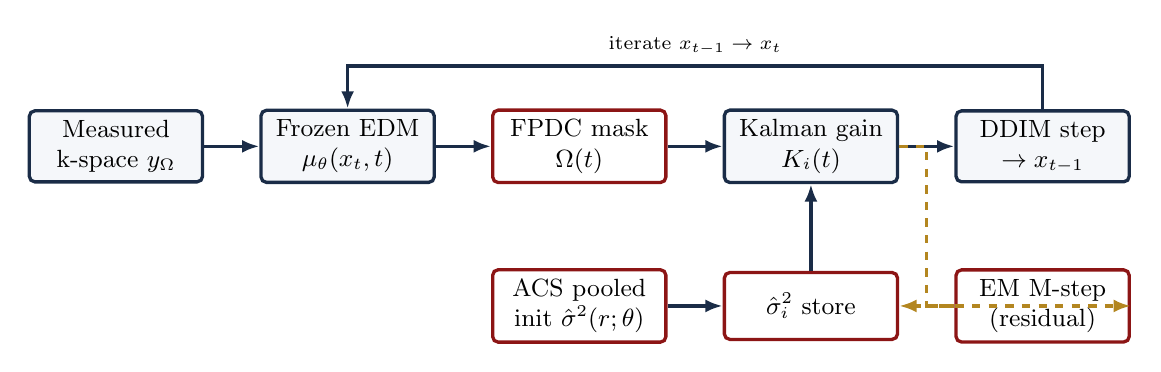
\begin{tikzpicture}[
      box/.style={draw=deepnavy, rounded corners=2pt, fill=softgray, very thick,
                  align=center, minimum width=2.20cm, minimum height=0.85cm,
                  font=\small},
      fakgdbox/.style={draw=stanfordred, rounded corners=2pt, fill=white, very thick,
                  align=center, minimum width=2.20cm, minimum height=0.85cm,
                  font=\small},
      arrow/.style={-{Latex[length=2.2mm]}, very thick, draw=deepnavy},
      feedback/.style={-{Latex[length=2.2mm]}, very thick, draw=accentgold, dashed}
    ]
      % --- main left-to-right pipeline (top row) ---
      \node[box]                              (y)       {Measured\\k-space $y_\Omega$};
      \node[box, right=0.7cm of y]            (denoise) {Frozen EDM\\$\muth(x_t,t)$};
      \node[fakgdbox, right=0.7cm of denoise] (fpdc)    {FPDC mask\\$\Omega(t)$};
      \node[box, right=0.7cm of fpdc]         (gain)    {Kalman gain\\$K_i(t)$};
      \node[box, right=0.7cm of gain]         (step)    {DDIM step\\$\to x_{t-1}$};

      \draw[arrow] (y)       -- (denoise);
      \draw[arrow] (denoise) -- (fpdc);
      \draw[arrow] (fpdc)    -- (gain);
      \draw[arrow] (gain)    -- (step);

      % --- iterate loop, drawn above the row to avoid crossings ---
      \draw[arrow] (step.north) -- ++(0,0.55) -| node[above, pos=0.25, font=\scriptsize] {iterate $x_{t-1} \to x_t$} (denoise.north);

      % --- calibration / feedback below the gain ---
      \node[fakgdbox, below=1.1cm of gain]  (sigma)  {$\hatsig_i^2$ store};
      \node[fakgdbox, left=0.7cm of sigma]  (acs)    {ACS pooled\\init $\hatsig^2(r;\theta)$};
      \node[fakgdbox, right=0.7cm of sigma] (mstep)  {EM M-step\\(residual)};

      \draw[arrow] (acs)    -- (sigma);
      \draw[arrow] (sigma)  -- (gain);
      \draw[feedback] (gain.east) -- ++(0.35,0) |- (mstep.east);
      \draw[feedback] (mstep) -- (sigma);
    \end{tikzpicture}
  \end{center}
  \vspace{0.2em}
  \footnotesize
  Top row: \PIGDM{}'s posterior-correction scaffold. Red boxes: \FAKGD{} components. Gold dashed loop: the closed-loop $\hatsig_i^2$ calibration \PIGDM{} lacks.
\end{frame}

% -----------------------------------------------------------
\begin{frame}{Component 1: frequency-aware Kalman gain}
  \small
  \begin{columns}[T]
    \begin{column}{0.55\textwidth}
      \textbf{\PIGDM{} update.} For $\mathbf{R}=\sigma_y^2 \mathbf{I}$:
      \[
        \hat{x}_{t-1} = \muth(x_t) + r_t \mathbf{A}^\top
        \!\left(\mathbf{A}\mathbf{A}^\top + \tfrac{\sigma_y^2}{\sigma_t^2}\mathbf{I}\right)^{-1}\!\!(y-\mathbf{A}\muth(x_t)).
      \]
      Right scaffold, wrong covariance.

      \vspace{0.4em}
      \textbf{\FAKGD{} substitution.} Use a diagonal $\hatR=\mathrm{diag}(\hatsig_i^2)$ from the ACS lines; the gain collapses to a per-frequency scalar:
      \[
        \boxed{K_i(t) = \frac{\sigma_t^2}{\sigma_t^2 + \hatsig_i^2}}
      \]
      \[
        \hat{x}_{t-1} = \muth(x_t) + \mathbf{F}_\Omega^\mathsf{H} K(t)\,\bigl(y_\Omega - \mathbf{F}_\Omega\muth(x_t)\bigr).
      \]
    \end{column}
    \begin{column}{0.45\textwidth}
      \textbf{Analytic radial noise model.} g-factor profiles are smooth in $r=\|\omega\|$; fit
      \[
        \hatsig^2(r;\theta) = \theta_0 + \theta_1 (r/r_{\max})^2 + \theta_2 (r/r_{\max})^4
      \]
      by weighted LS against the ACS residuals.

      \vspace{0.4em}
      \textbf{Why this gain shape.}
      \begin{itemize}
        \item $\sigma_t \gg \hatsig_i$ (early): $K_i \!\to\! 1$, trust the measurement.
        \item $\sigma_t \ll \hatsig_i$ (late): $K_i \!\to\! 0$, trust the prior.
        \item Three parameters per volume; no extra scan, no retraining.
      \end{itemize}
    \end{column}
  \end{columns}
\end{frame}

% -----------------------------------------------------------
\begin{frame}{Component 2: frequency-progressive data consistency}
  \small
  \begin{columns}[T]
    \begin{column}{0.50\textwidth}
      \textbf{Failure mode: DC shock.}
      Hard DC forces $[\mathbf{F}_\Omega \hat{x}_{t-1}]_i = y_i$ at \emph{every} frequency on \emph{every} step. The denoiser at step $t{-}1$ expects noise level $\sigma_{t-1}$; zeroing the residual locally creates a distributional mismatch that injects Gibbs-like ringing.

      \vspace{0.4em}
      \textbf{FPDC schedule.} Enforce DC only inside an expanding radius:
      \[
        r(t) = r_{\text{ACS}} + (r_{\max}-r_{\text{ACS}})\,(1-t/T)^\beta,
      \]
      $\Omega(t) = \{i \in \Omega : \|\omega_i\| \leq r(t)\}$.
      Defaults: $\beta = 1$, ACS radius from the mask.
    \end{column}
    \begin{column}{0.50\textwidth}
      \begin{center}
        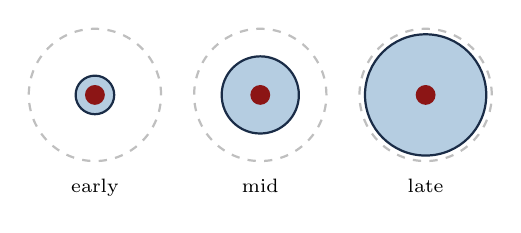
\begin{tikzpicture}[scale=0.70, every node/.style={font=\scriptsize}]
          \foreach \i/\rad/\lab in {1/0.35/early, 2/0.70/mid, 3/1.10/late}{
            \begin{scope}[xshift={(\i-2)*3.0cm}]
              \draw[thick, gray!50, dashed] (0,0) circle (1.2);
              \fill[softblue!40] (0,0) circle (\rad);
              \draw[draw=deepnavy, thick] (0,0) circle (\rad);
              \fill[stanfordred] (0,0) circle (0.18);
              \node[below=0.10cm] at (0,-1.2) {\lab};
            \end{scope}}
        \end{tikzpicture}
      \end{center}
      \footnotesize
      Blue disk: active frequencies $\Omega(t)$. Red core: ACS, always on. Dashed: $r_{\max}$.
    \end{column}
  \end{columns}
\end{frame}

% -----------------------------------------------------------
\begin{frame}{Component 3: M-step and the $\gamma$-family}
  \small
  After each $\muth(x_t)$ we refine $\hatsig_i^2$ from the residual energy
  $r_i^{(t)} = y_i - [\mathbf{F}_{\Omega(t)}\muth(x_t)]_i$:
  \[
    \hatsig_i^2 \leftarrow \alpha(t)\,\hatsig_i^2 + (1-\alpha(t))\,\max\!\left(|r_i^{(t)}|^2 - \gamma\,\sigma_t^2,\ \epsilon\right).
  \]
  \begin{columns}[T]
    \begin{column}{0.55\textwidth}
      \textbf{The bias question.} Residual energy mixes measurement noise and denoiser error. For error fraction $\eta^2 \ll 1$:
      \[
        \mathbb{E}\!\left[|r_i^{(t)}|^2\right] = \hatsig_i^2 + \eta^2 \sigma_t^2.
      \]
      ``Obvious'' fix: subtract the full $\sigma_t^2$ ($\gamma=1$). This over-corrects by $1/\eta^2$, drives $\hatsig_i^2 \to 0$, and collapses $K_i \to 1$ everywhere.
    \end{column}
    \begin{column}{0.45\textwidth}
      \textbf{Oracle result ($R{=}4$, $T{=}100$).}
      \begin{center}
      \scriptsize
      \begin{tabular}{@{}l c c@{}}
        \toprule
        Variant & PSNR (dB) & $\Delta$ vs.\ \PIGDM{} \\
        \midrule
        \PIGDM{} (isotropic) & 60.2 & --- \\
        \FAKGD{} $\gamma{=}0$ (safe) & 60.9 & $+0.7$ \\
        \FAKGD{} $\gamma{=}1$ (na\"ive) & 47.4 & $\mathbf{-12.8}$ \\
        \bottomrule
      \end{tabular}
      \end{center}
      \vspace{0.3em}
      \footnotesize
      Result is sampler-agnostic: any diffusion solver that estimates noise from residuals inherits the same bias.
    \end{column}
  \end{columns}
\end{frame}

% -----------------------------------------------------------
\begin{frame}{Component 4: FA-KGD-3D --- volumetric ACS pooling}
  \small
  \begin{columns}[T]
    \begin{column}{0.55\textwidth}
      \textbf{Observation.} Variable-density trajectories reacquire the same ACS region for every slice; receive-coil noise is stationary across $z$.

      \vspace{0.3em}
      \textbf{Estimator.} Pool the per-frequency sample variance across slices before the radial fit:
      \[
        \tilde\sigma_i^{2,\text{3D}} = \tfrac{1}{N_z(N_c-1)} \sum_{z,c} \bigl|y_{i,c,z} - \bar y_{i,z}\bigr|^2.
      \]
      Effective DOF: $N_c{-}1 \to N_z(N_c{-}1)$. Single pre-pass per volume, then $\hatsig^2(r;\theta)$ initialises the sampler for every slice.
    \end{column}
    \begin{column}{0.45\textwidth}
      \textbf{Empirical (16-slice brain).}
      \begin{itemize}
        \item Per-slice $\hatsig_i^2$: \alert{26\%} rel.\ RMSE.
        \item Pooled $\hatsig_i^2$: \alert{6.3\%} rel.\ RMSE ($\sim 17\times$ MSE reduction, matches theoretical $N_z{=}16$).
        \item Radial fit ($K{=}2$): \alert{0.8\%} mean rel.\ error on the full grid; statistically indistinguishable from an oracle.
      \end{itemize}
      \vspace{0.3em}
      \footnotesize
      No new weights, no per-step overhead --- the only change is one pre-pass.
    \end{column}
  \end{columns}
\end{frame}

% -----------------------------------------------------------
\begin{frame}{Preliminary quantitative results}
  \footnotesize
  \begin{columns}[T]
    \begin{column}{0.66\textwidth}
      \centering
      \setlength{\tabcolsep}{3pt}
      \scriptsize
      \begin{tabular}{@{}l c ccc c ccc@{}}
        \toprule
        \multirow{2}{*}{Setting} & \multirow{2}{*}{$T$}
          & \multicolumn{3}{c}{PSNR (dB) $\uparrow$} & \phantom{x}
          & \multicolumn{3}{c}{SSIM $\uparrow$} \\
        \cmidrule{3-5} \cmidrule{7-9}
         & & DPS & \PIGDM{} & \textbf{\FAKGD{}} &
         & DPS & \PIGDM{} & \textbf{\FAKGD{}} \\
        \midrule
        Brain $R{=}4$ & 20 & 27.31 & 29.43 & \textbf{29.73} & & .663 & .867 & \textbf{.871} \\
        Brain $R{=}4$ & 50 & 28.07 & 30.00 & \textbf{30.49} & & .721 & .864 & \textbf{.874} \\
        Knee $R{=}4$  & 20 & 28.57 & 29.05 & \textbf{29.19} & & .655 & .645 & \textbf{.658} \\
        Knee $R{=}8$  & 20 & 28.51 & 28.67 & \textbf{28.79} & & .646 & .630 & \textbf{.642} \\
        \bottomrule
      \end{tabular}

      \vspace{0.3em}
      {\scriptsize fastMRI multi-coil, frozen EDM checkpoint, mean over 5 validation volumes per setting.}
    \end{column}
    \begin{column}{0.33\textwidth}
      \begin{itemize}
        \item \FAKGD{} $>$ \PIGDM{} in every cell ($+0.12$ to $+0.50$~dB).
        \item Brain $2$--$3\times$ knee --- prior accuracy matters.
        \item Supervised E2E-VarNet sits $\sim$10~dB higher; multicoil raw data, separate axis.
      \end{itemize}
    \end{column}
  \end{columns}
\end{frame}

% -----------------------------------------------------------
\begin{frame}{Scaling with step budget: the regression \PIGDM{} can't avoid}
  \begin{columns}[T]
    \begin{column}{0.55\textwidth}
      \begin{center}
        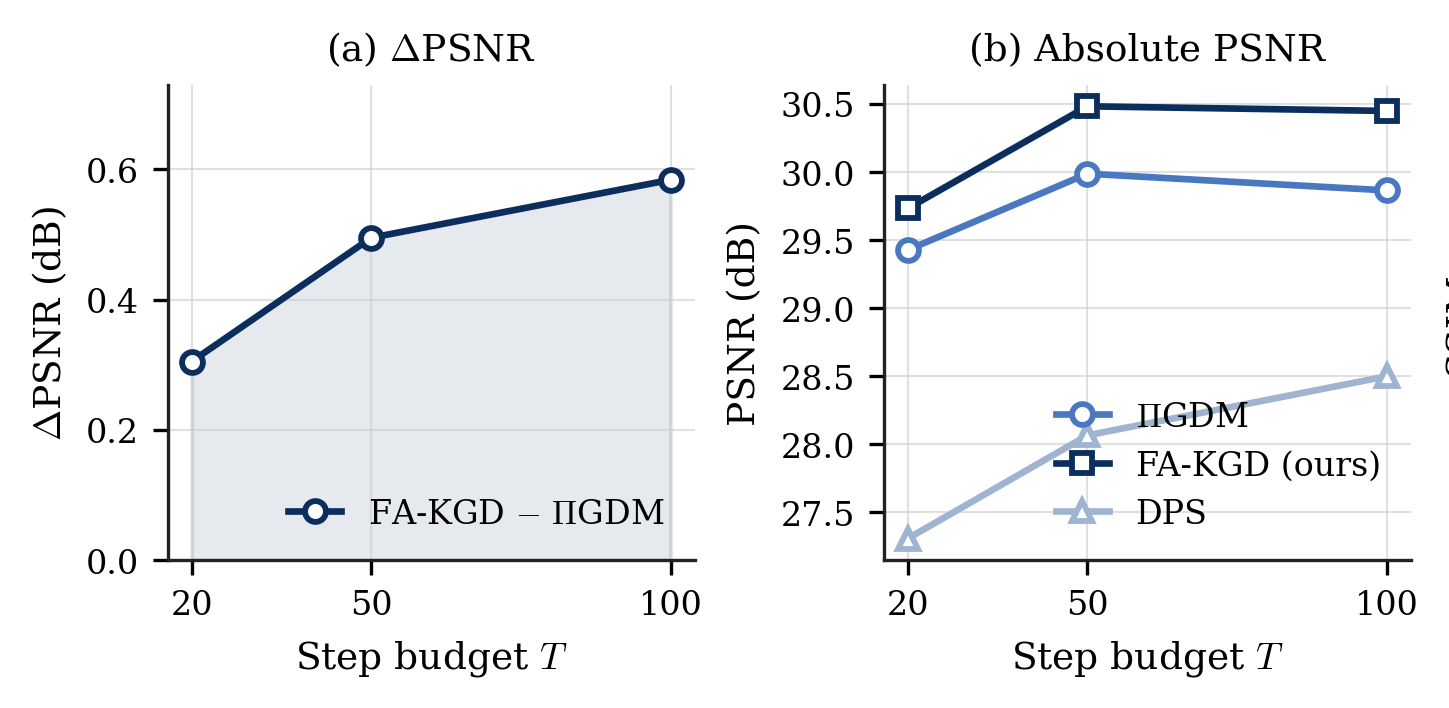
\includegraphics[width=\textwidth]{fig3_scaling_curve_ab.png}
      \end{center}
      \vspace{-0.4em}
      \footnotesize
      Brain $R{=}4$. \PIGDM{} peaks at $T{=}50$ and regresses; \FAKGD{} stays flat.
    \end{column}
    \begin{column}{0.45\textwidth}
      \scriptsize
      \textbf{At scale} (192 slices, 12 volumes, paired Wilcoxon $p<10^{-30}$):
      \begin{center}
      \begin{tabular}{@{}c c c c@{}}
        \toprule
        $R$ & $T$ & \PIGDM{} & $\Delta$ \FAKGD{} \\
        \midrule
        4 & 20  & 29.83 & $+0.23$ \\
        4 & 50  & 29.85 & $+0.39$ \\
        4 & 100 & \alert{29.38} & $\mathbf{+0.51}$ \\
        \midrule
        8 & 20  & 27.14 & $+0.11$ \\
        8 & 50  & 27.13 & $+0.19$ \\
        8 & 100 & \alert{26.65} & $\mathbf{+0.25}$ \\
        \bottomrule
      \end{tabular}
      \end{center}
      \vspace{0.2em}
      \footnotesize
      \FAKGD{} grows with $T$, \PIGDM{} decays with $T$ --- both signatures of DC shock.
    \end{column}
  \end{columns}
\end{frame}

% -----------------------------------------------------------
\begin{frame}{Where the gains live: frequency-band + cross-domain}
  \begin{columns}[T]
    \begin{column}{0.50\textwidth}
      
\includegraphics[width=\textwidth]{fig4_frequency_analysis.png}

      \vspace{-0.3em}
      \footnotesize
      Per-band k-space NMSE, brain $R{=}4$. Gains in low/mid bands, $\sim 0$ at high bands --- the FPDC signature.
    \end{column}
    \begin{column}{0.49\textwidth}
      
\includegraphics[width=\textwidth]{fig7_cross_domain_bar.png}

      \vspace{-0.3em}
      \footnotesize
      Cross-domain: brain (matched) gains $2$--$3\times$ knee (transfer).
    \end{column}
  \end{columns}
\end{frame}

% -----------------------------------------------------------
\begin{frame}{Component ablation: superadditive synergy}
  \small
  \begin{columns}[T]
    \begin{column}{0.50\textwidth}
      Oracle denoiser ($\eta{=}0.1$) decouples score error from sampler choices, $R{=}4$, $T{=}100$:
      \begin{center}
      \scriptsize
      \begin{tabular}{@{}l c c@{}}
        \toprule
        Variant & PSNR & $\Delta$ \\
        \midrule
        \PIGDM{} (isotropic) & 60.2 & --- \\
        \PIGDM{} $+$ FPDC only & 60.2 & $+0.0$ \\
        \FAKGD{}-EM only ($\gamma{=}0$) & 60.9 & $+0.7$ \\
        \textbf{Full method} & \textbf{62.1} & $\mathbf{+1.9}$ \\
        \bottomrule
      \end{tabular}
      \end{center}
    \end{column}
    \begin{column}{0.50\textwidth}
      \begin{itemize}
        \item FPDC alone $\to 0$~dB: isotropic gain ignores the gate.
        \item Gain alone $\to +0.7$~dB: capped by DC-shock-polluted residuals.
        \item Joint $\to +1.9$~dB, $1.2$~dB above the sum.
      \end{itemize}
      The two components are \emph{mutually enabling}; this is what \FAKGD{} adds over treating them independently.
    \end{column}
  \end{columns}
\end{frame}

% -----------------------------------------------------------
\begin{frame}{Setup and remaining work}
  \small
  \begin{columns}[T]
    \begin{column}{0.50\textwidth}
      \textbf{Experimental setup.}
      \begin{itemize}
        \item fastMRI multi-coil brain (AXT2) and knee.
        \item Frozen public EDM checkpoint; no task-specific training.
        \item $R \in \{4,8\}$ variable-density, $24{\times}24$ ACS.
        \item PSNR / SSIM vs.\ fully-sampled GT; paired Wilcoxon at scale.
        \item Defaults $\beta{=}1$, $\alpha_0{=}0.95$, $\gamma{=}0$.
      \end{itemize}
    \end{column}
    \begin{column}{0.50\textwidth}
      \textbf{Remaining for the final report.}
      \begin{itemize}
        \item Knee-matched EDM checkpoint, to test the score-prior hypothesis directly.
        \item Multi-coil SENSE (RSS today; closes part of the supervised gap).
        \item Failure-case gallery and limitations write-up.
      \end{itemize}
    \end{column}
  \end{columns}
\end{frame}

% -----------------------------------------------------------
\begin{frame}[allowframebreaks]{References}
  \scriptsize
  \begin{thebibliography}{10}
    \bibitem{song2023pigdm}
      J.~Song et al.\ Pseudoinverse-Guided Diffusion Models for Inverse Problems. \emph{ICLR}, 2023.
    \bibitem{chung2023dps}
      H.~Chung et al.\ Diffusion Posterior Sampling for General Noisy Inverse Problems. \emph{ICLR}, 2023.
    \bibitem{kawar2022ddrm}
      B.~Kawar et al.\ Denoising Diffusion Restoration Models. \emph{NeurIPS}, 2022.
    \bibitem{karras2022edm}
      T.~Karras et al.\ Elucidating the Design Space of Diffusion-Based Generative Models. \emph{NeurIPS}, 2022.
    \bibitem{daras2025adps}
      G.~Daras et al.\ Ambient Diffusion Posterior Sampling. \emph{ICLR}, 2025.
    \bibitem{uecker2014espirit}
      M.~Uecker et al.\ ESPIRiT: An Eigenvalue Approach to Autocalibrating Parallel MRI. \emph{MRM}, 71(3):990--1001, 2014.
    \bibitem{zbontar2018fastmri}
      J.~Zbontar et al.\ fastMRI: An Open Dataset and Benchmarks for Accelerated MRI. \emph{arXiv:1811.08839}, 2018.
    \bibitem{sriram2020varnet}
      A.~Sriram et al.\ End-to-End Variational Networks for Accelerated MRI Reconstruction. \emph{MICCAI}, 2020.
    \bibitem{jalal2021robust}
      A.~Jalal et al.\ Robust Compressed Sensing MRI with Deep Generative Priors. \emph{NeurIPS}, 2021.
    \bibitem{chung2022scoremri}
      H.~Chung, J.~C.~Ye.\ Score-Based Diffusion Models for Accelerated MRI. \emph{Medical Image Analysis}, 2022.
  \end{thebibliography}
\end{frame}

\end{document}
